\listoffigures
\addcontentsline{toc}{chapter}{図目次}

\begin{figure}
    \centering
    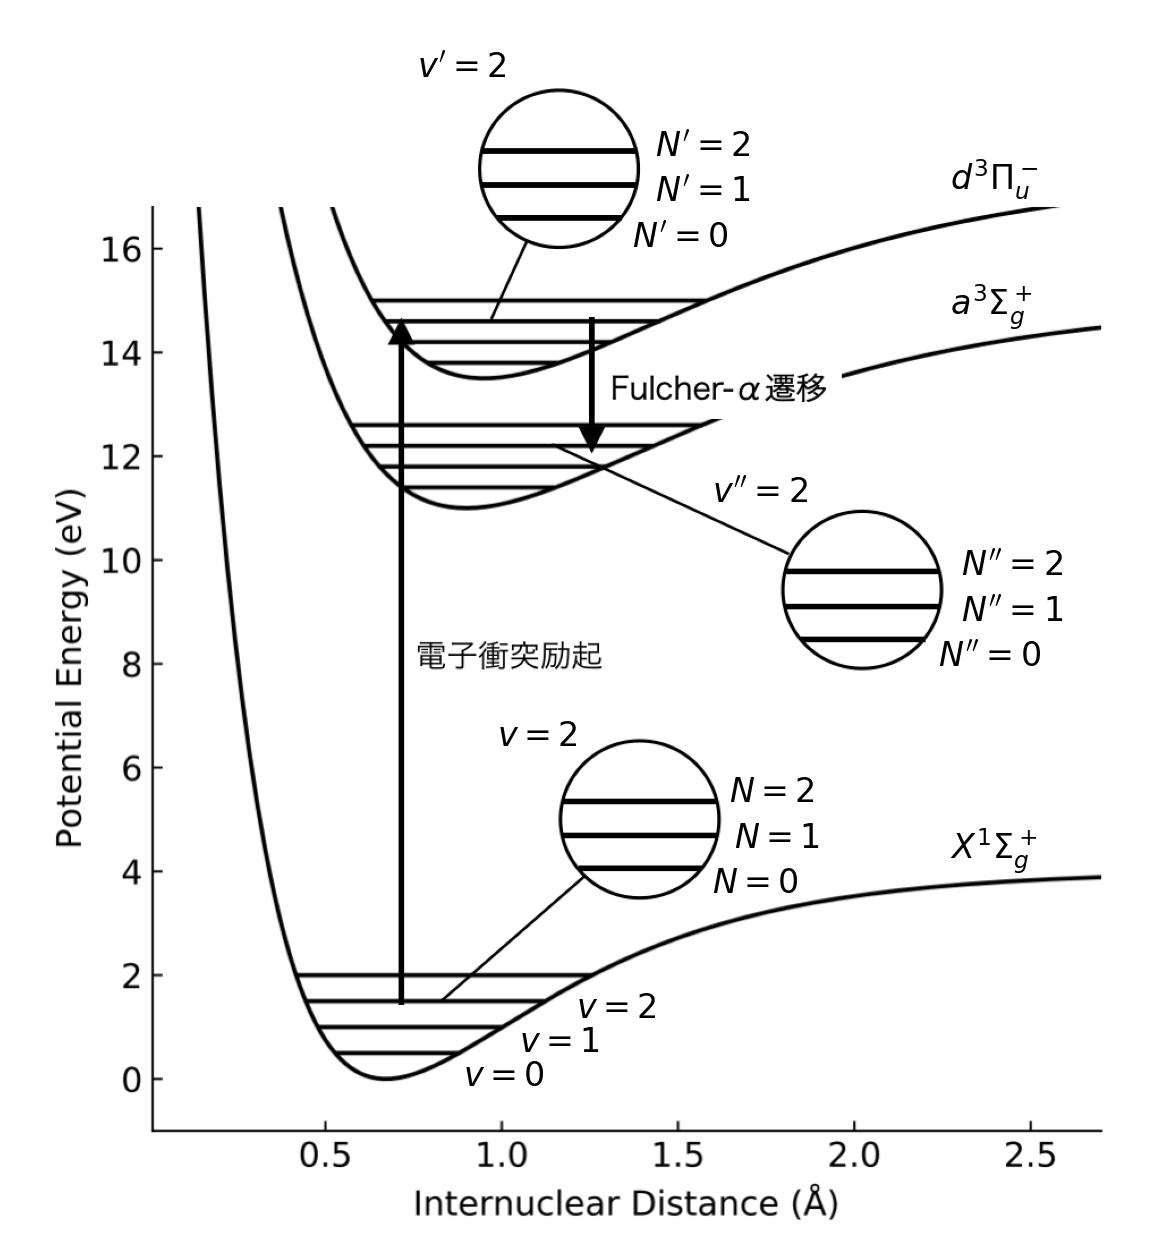
\includegraphics[width=15cm]{pictures/energy-level.png}
    \caption{$\rm{H}_2$のポテンシャル曲線}
    \label{fig:energy-level}
\end{figure}

\begin{figure}
    \centering
    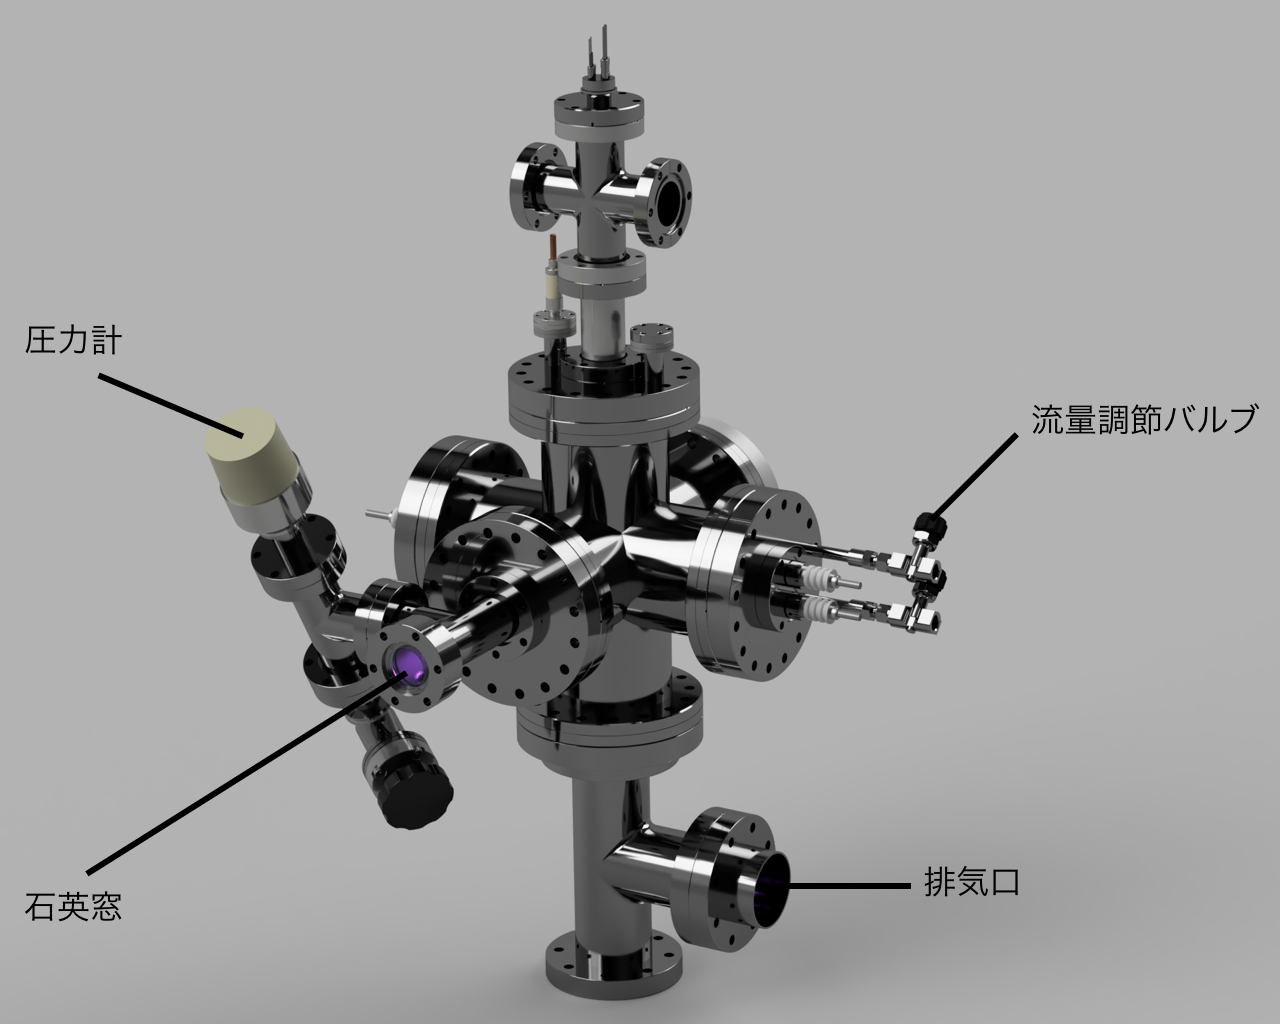
\includegraphics[width=15cm]{pictures/chamber-picture.png}
    \caption{プラズマチャンバの外観}
    \label{fig:chamber-picture}
\end{figure}

\begin{figure}
    \centering
    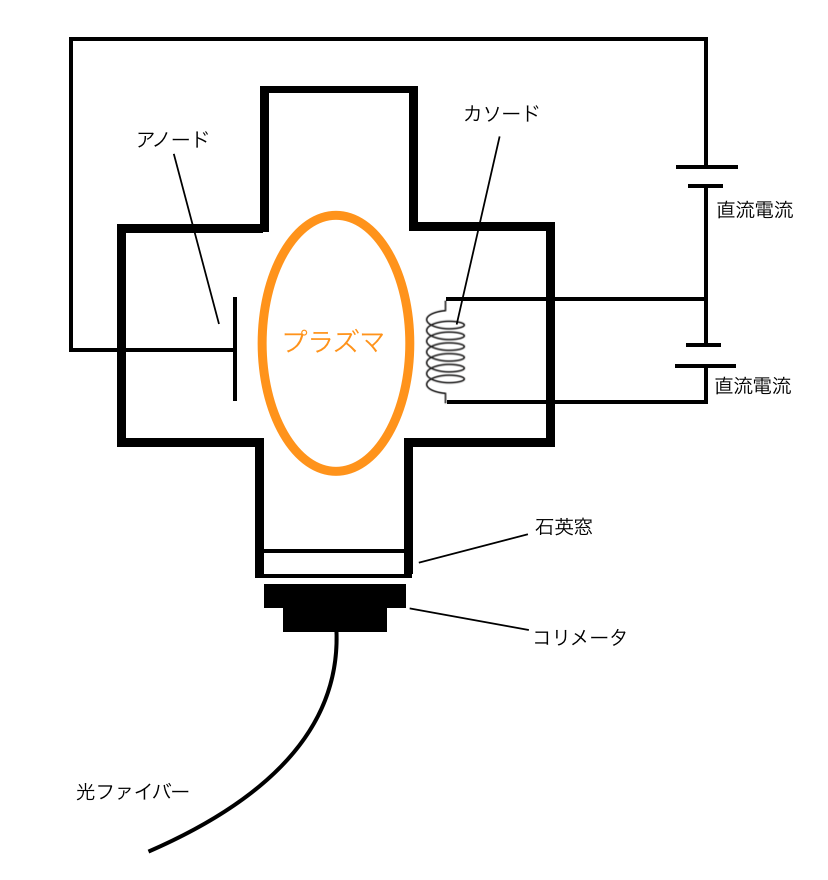
\includegraphics[width=15cm]{pictures/chamber-simple.png}
    \caption{プラズマチャンバの構造の簡略図}
    \label{fig:chamber-simple}
\end{figure}

\begin{figure}
    \centering
    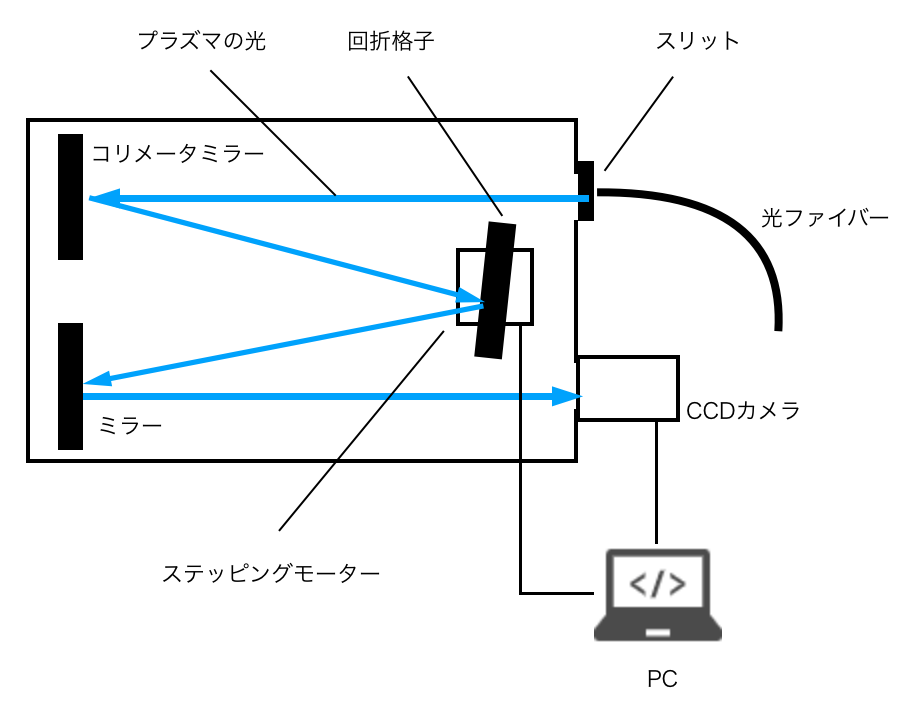
\includegraphics[width=15cm]{pictures/spectrometer-picture.png}
    \caption{分光器の概略図}
    \label{fig:spectrometer-picture}
\end{figure}

\begin{figure}
    \centering
    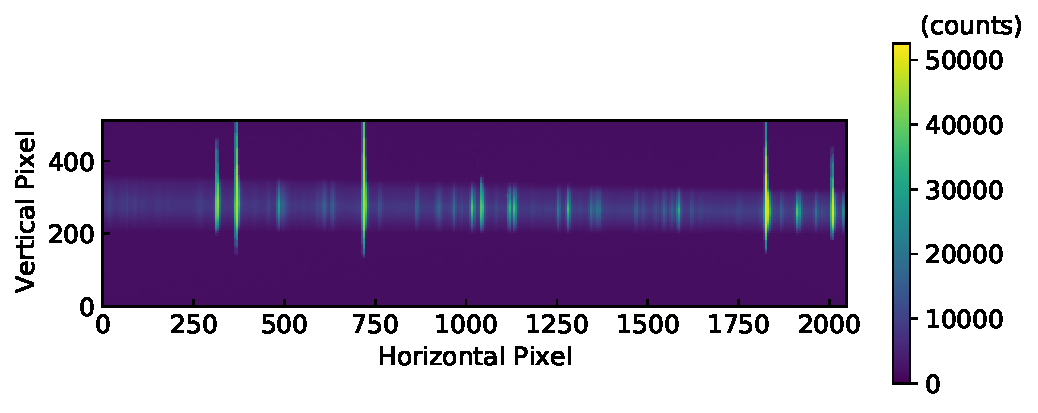
\includegraphics[width=15cm]{pictures/picture-example.pdf}
    \caption{CCDカメラで撮影したスペクトルの例}
    \label{fig:picture-example}
\end{figure}

\begin{figure}
    \centering
    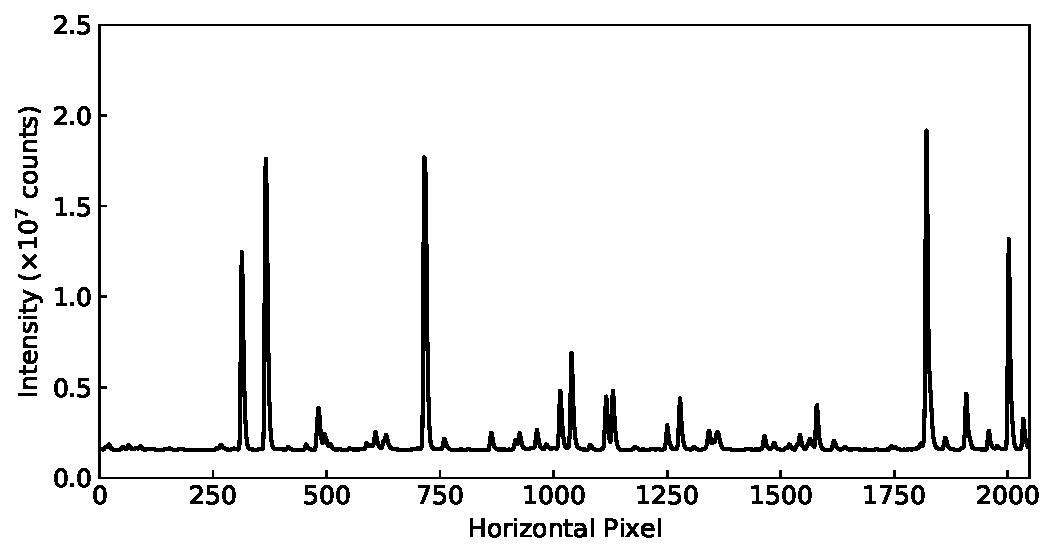
\includegraphics[width=15cm]{pictures/spectrum-example.pdf}
    \caption{図\ref{fig:picture-example}の各画素のカウント数を縦に合計した図}
    \label{fig:spectrum-example}
\end{figure}

\begin{figure}
    \centering
    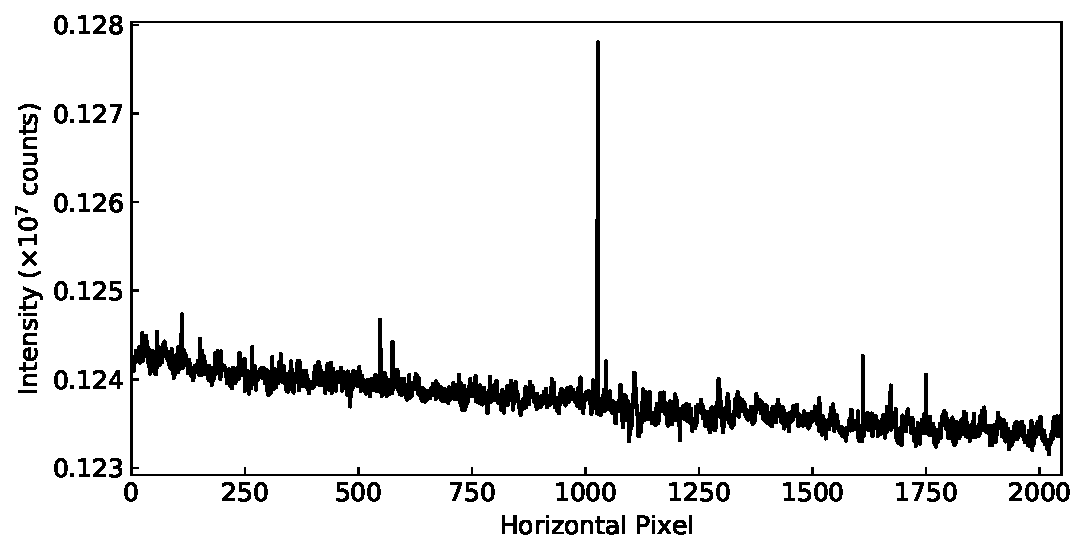
\includegraphics[width=15cm]{pictures/back-spectrum-example.pdf}
    \caption{プラズマを消した状態で得た画像の各画素のカウント数を縦に合計した図}
    \label{fig:back-spectrum-example}
\end{figure}

\begin{figure}
    \centering
    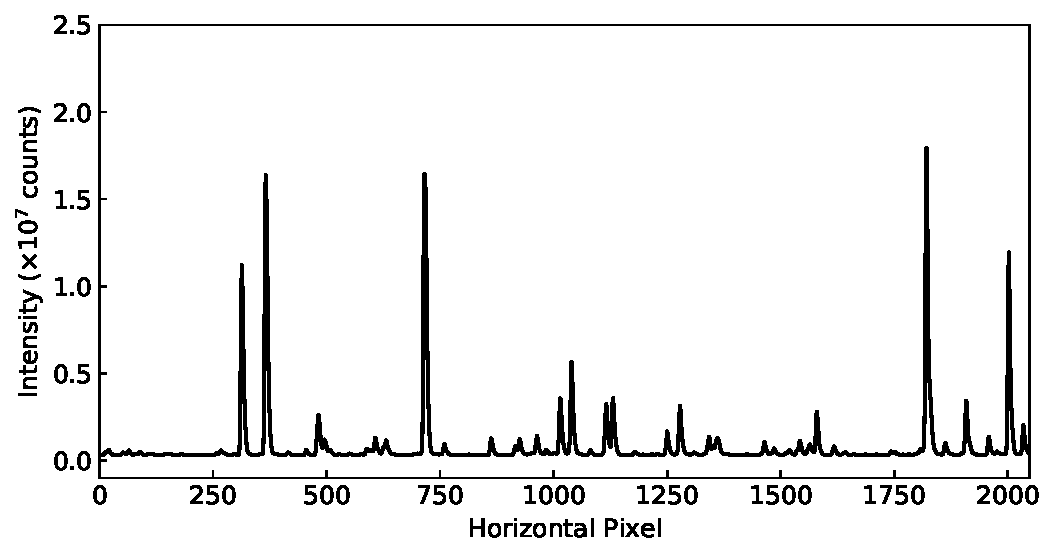
\includegraphics[width=15cm]{pictures/true-spectrum-example.pdf}
    \caption{図\ref{fig:spectrum-example}のカウント数から図\ref{fig:back-spectrum-example}のカウント数を減算した図}
    \label{fig:true-spectrum-example}
\end{figure}

\begin{figure}
    \centering
    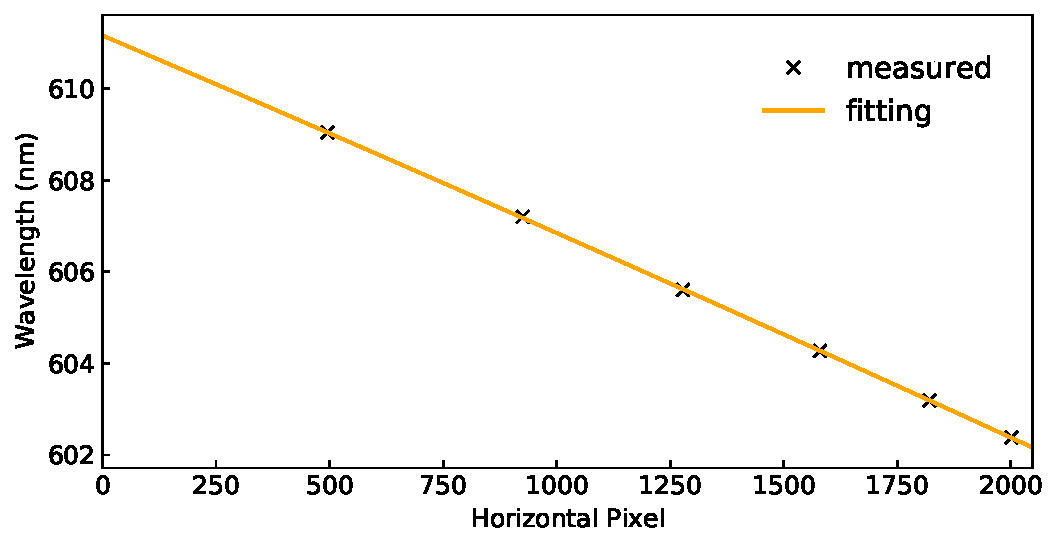
\includegraphics[width=15cm]{pictures/pixel-to-wavelength.pdf}
    \caption{ピクセルと波長の関係の例}
    \label{fig:pixel-to-wavelength}
\end{figure}

\begin{figure}
    \centering
    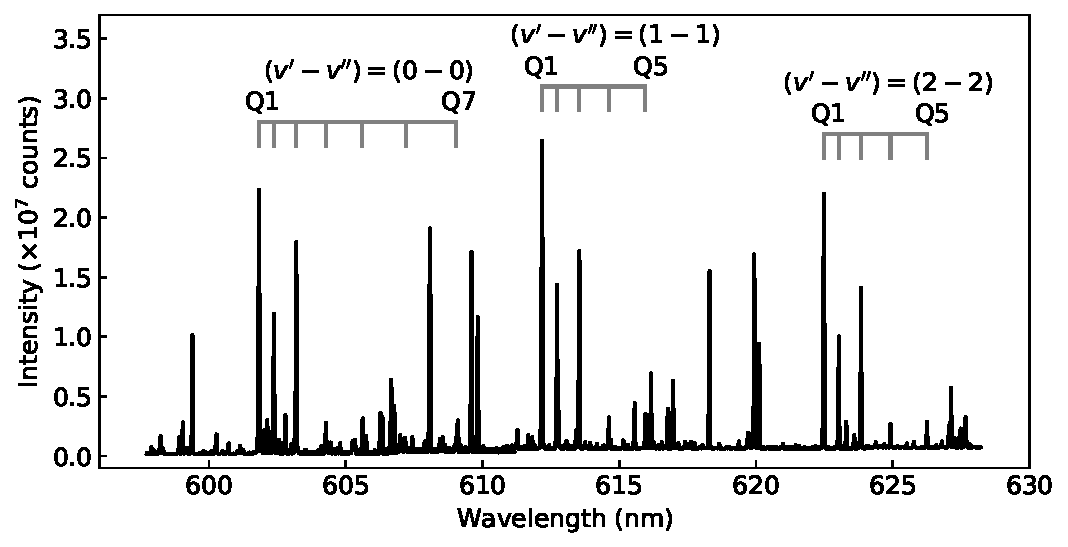
\includegraphics[width=15cm]{pictures/all-spectrum.pdf}
    \caption{Fulcher-α帯Q枝発光スペクトル}
    \label{fig:all-spectrum}
\end{figure}

\begin{figure}
    \centering
    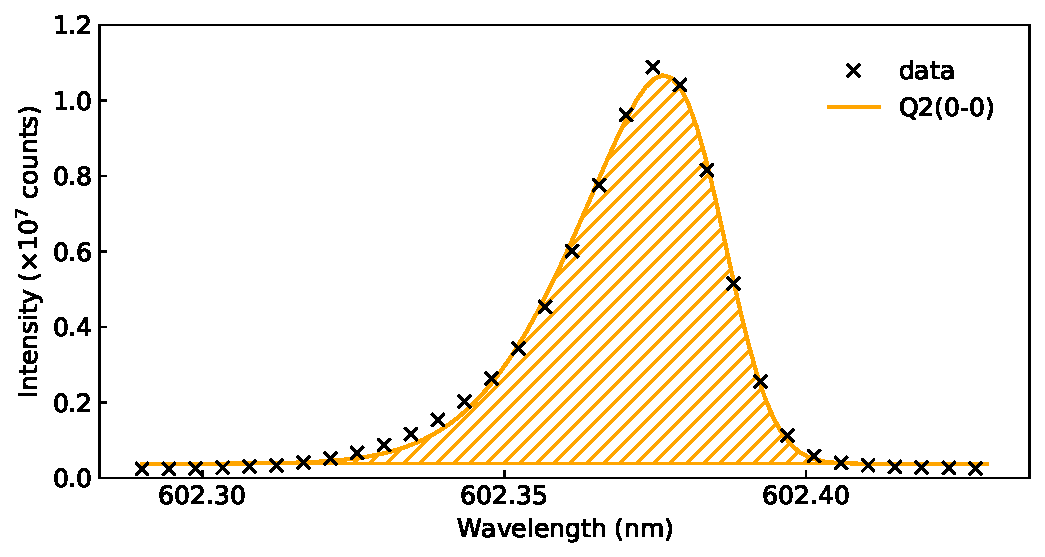
\includegraphics[width=15cm]{pictures/skewed-gaussian-fitting-00_Q2.pdf}
    \caption{Q2(0-0)発光線の歪正規分布関数によるフィッティング結果}
    \label{fig:voigt-fitting-1}
\end{figure}

\begin{figure}
    \centering
    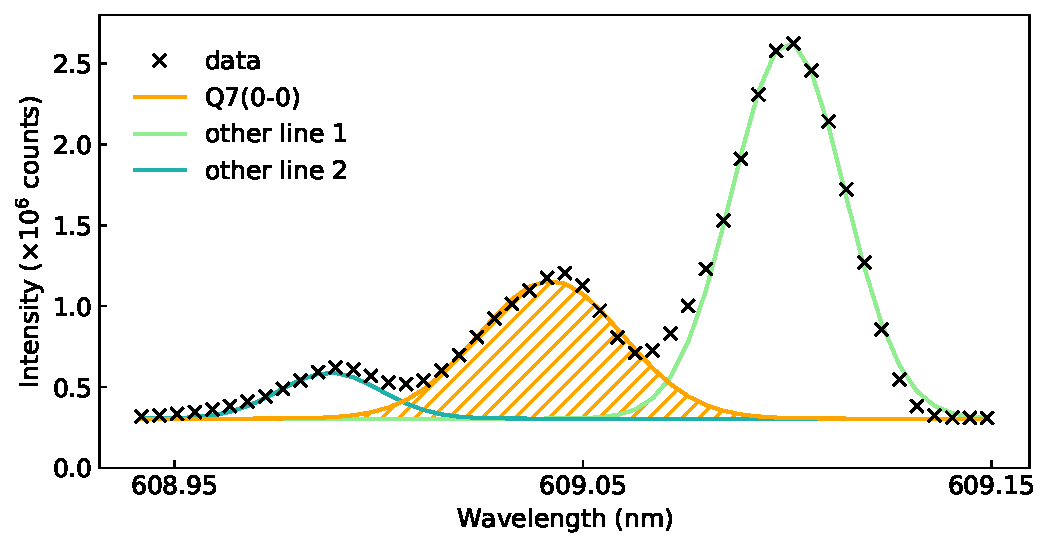
\includegraphics[width=15cm]{pictures/skewed-gaussian-fitting-00_Q7.pdf}
    \caption{Q7(0-0)発光線の歪正規分布関数フィッティングによる分離}
    \label{fig:voigt-fitting-2}
\end{figure}

\begin{figure}
    \centering
    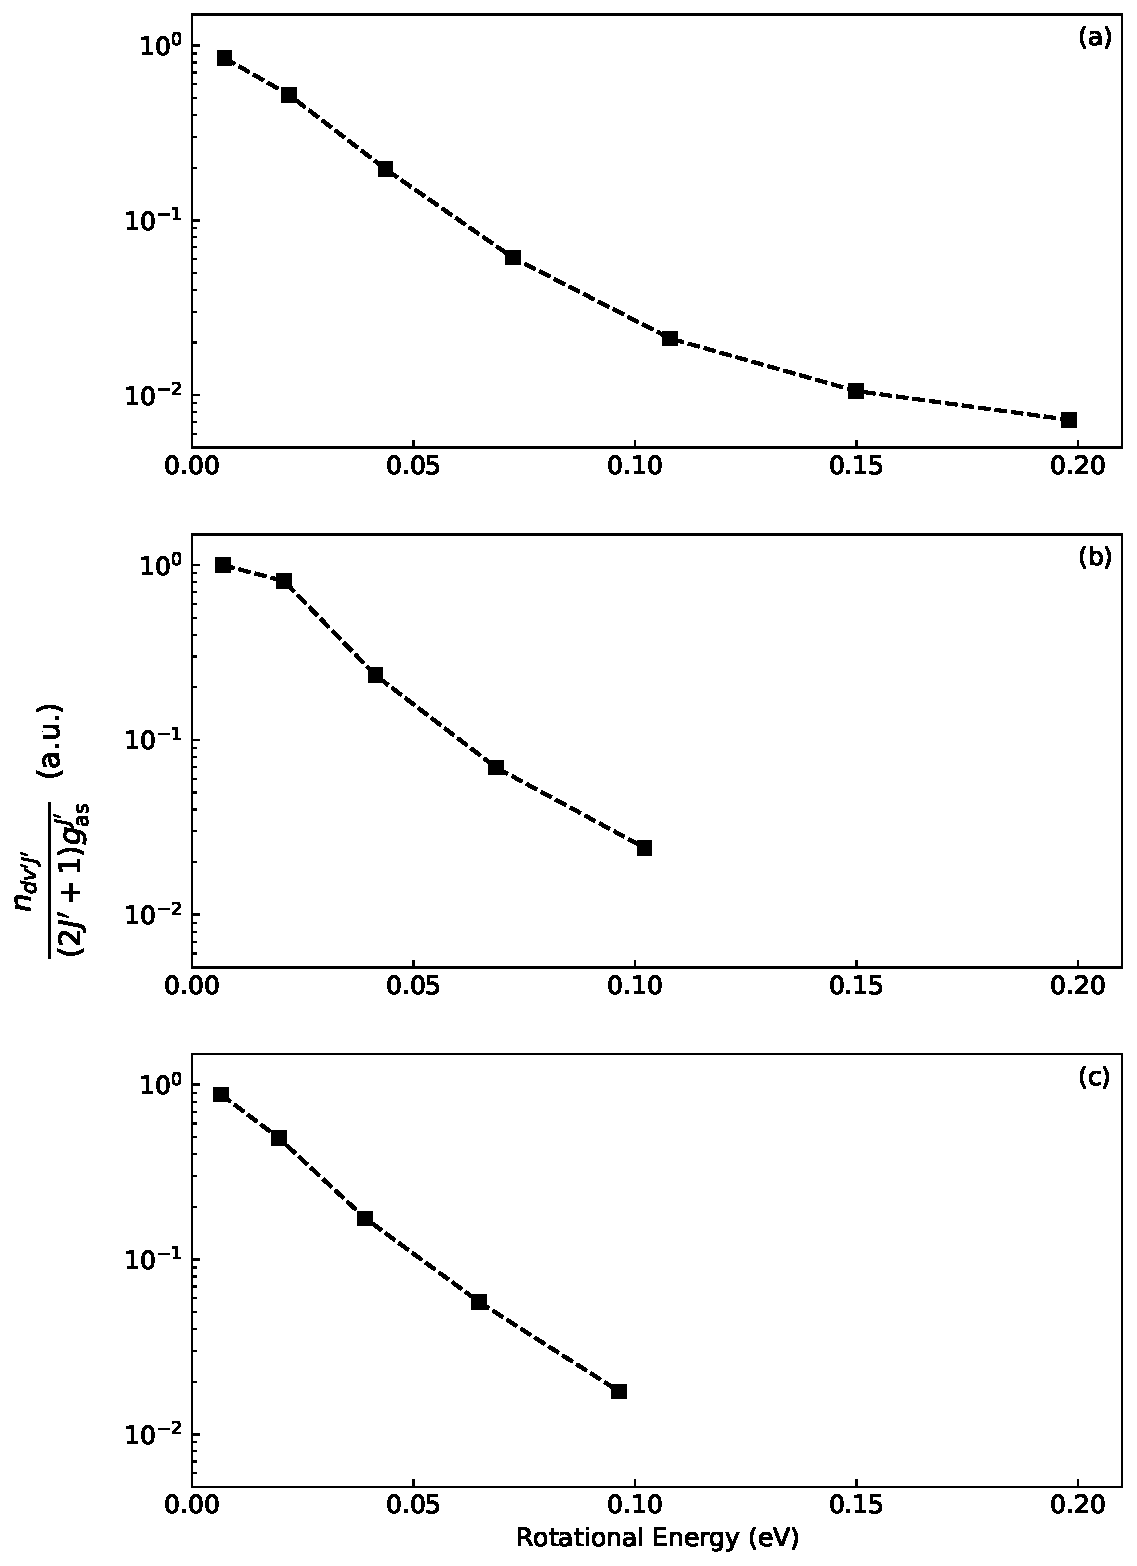
\includegraphics[width=15cm]{pictures/upper-boltzmann-plot.pdf}
    \caption{発光上準位における振動・回転状態占有率の回転エネルギー依存性}
    \label{fig:upper-boltzmann-plot}
\end{figure}

\begin{figure}
    \centering
    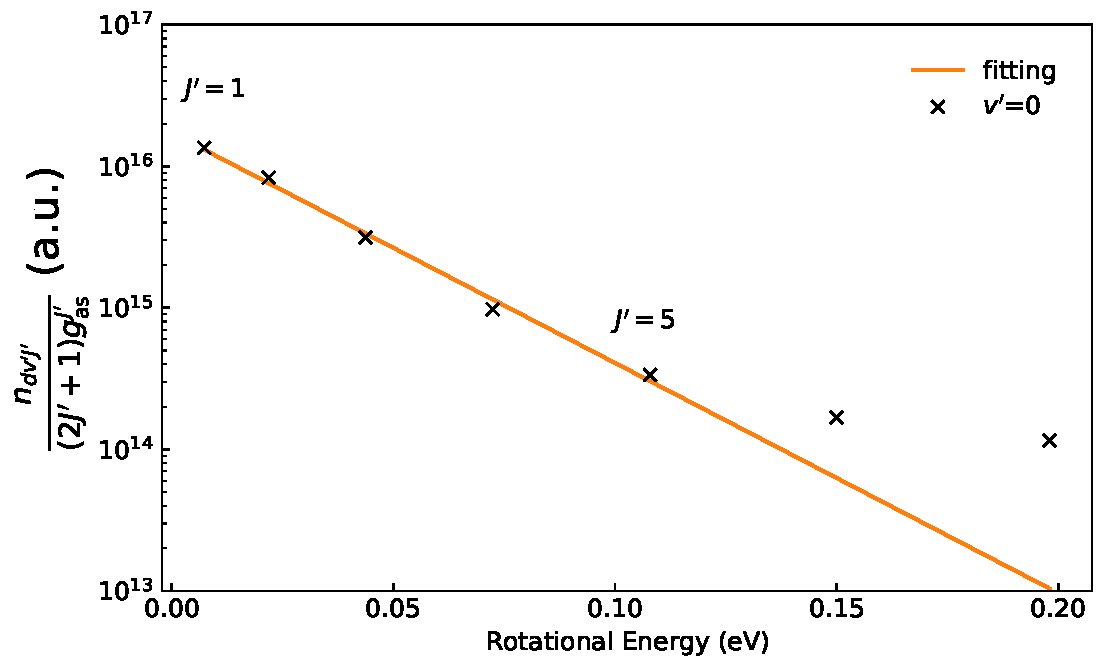
\includegraphics[width=15cm]{pictures/upper-fitting-0.pdf}
    \caption{発光上準位における振動・回転状態占有率のボルツマン分布によるフィッティング結果($v'=0$)}
    \label{fig:upper-fitting-0}
\end{figure}

\begin{figure}
    \centering
    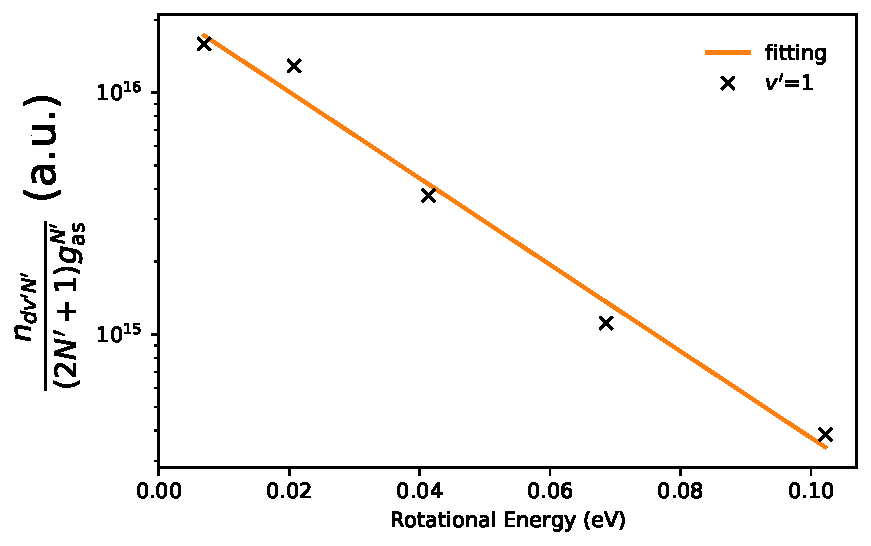
\includegraphics[width=15cm]{pictures/upper-fitting-1.pdf}
    \caption{発光上準位における振動・回転状態占有率のボルツマン分布によるフィッティング結果($v'=1$)}
    \label{fig:upper-fitting-1}
\end{figure}

\begin{figure}
    \centering
    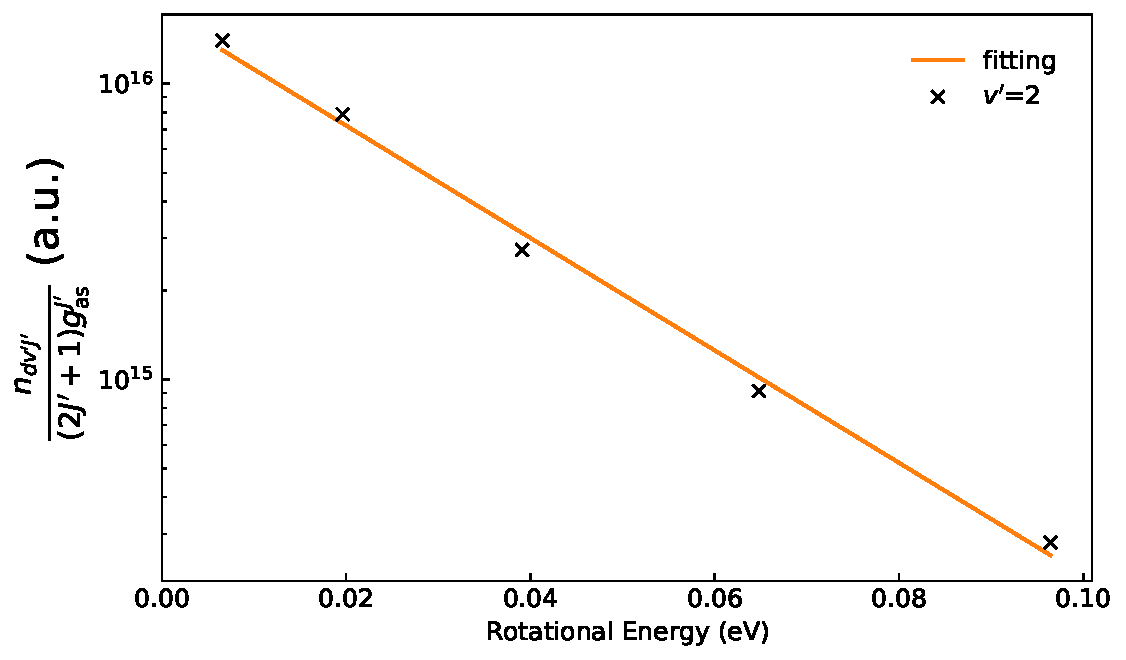
\includegraphics[width=15cm]{pictures/upper-fitting-2.pdf}
    \caption{発光上準位における振動・回転状態占有率のボルツマン分布によるフィッティング結果($v'=2$)}
    \label{fig:upper-fitting-2}
\end{figure}

\begin{figure}
    \centering
    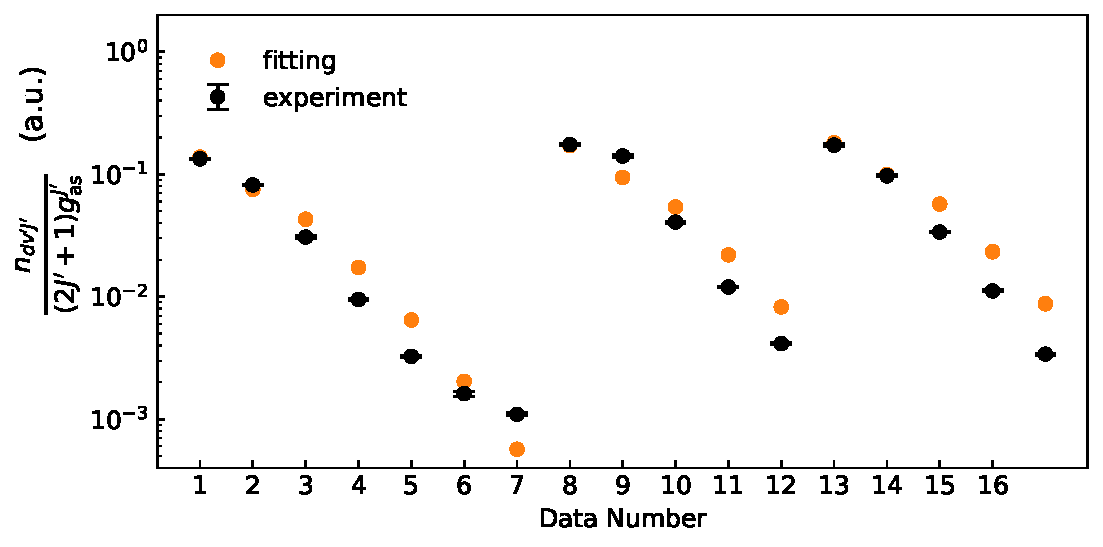
\includegraphics[width=15cm]{pictures/fitting-result.pdf}
    \caption{発光上準位における振動・回転状態占有率のコロナモデルによるフィッティング結果}
    \label{fig:fitting-result}
\end{figure}

\begin{figure}
    \centering
    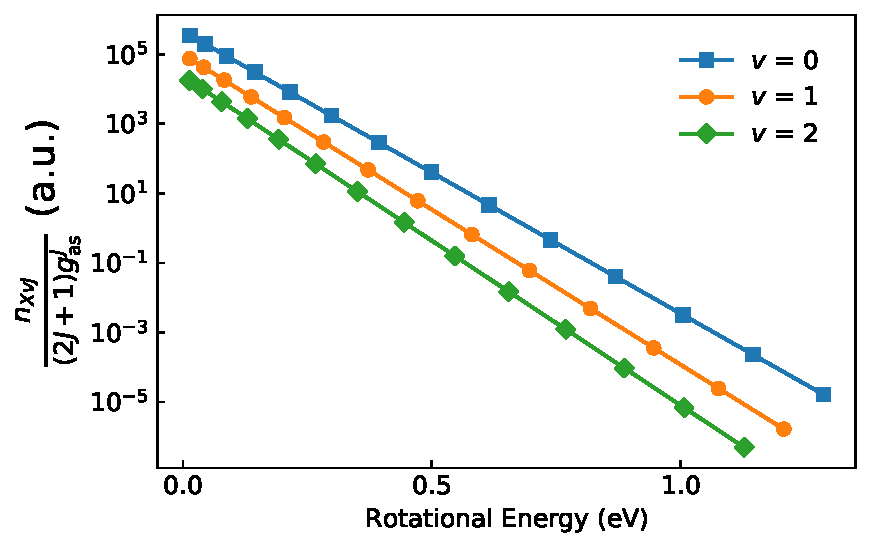
\includegraphics[width=15cm]{pictures/ground-state-n.pdf}
    \caption{基底準位における振動・回転状態占有率の回転エネルギー依存性}
    \label{fig:ground-state-n}
\end{figure}

\begin{figure}
    \centering
    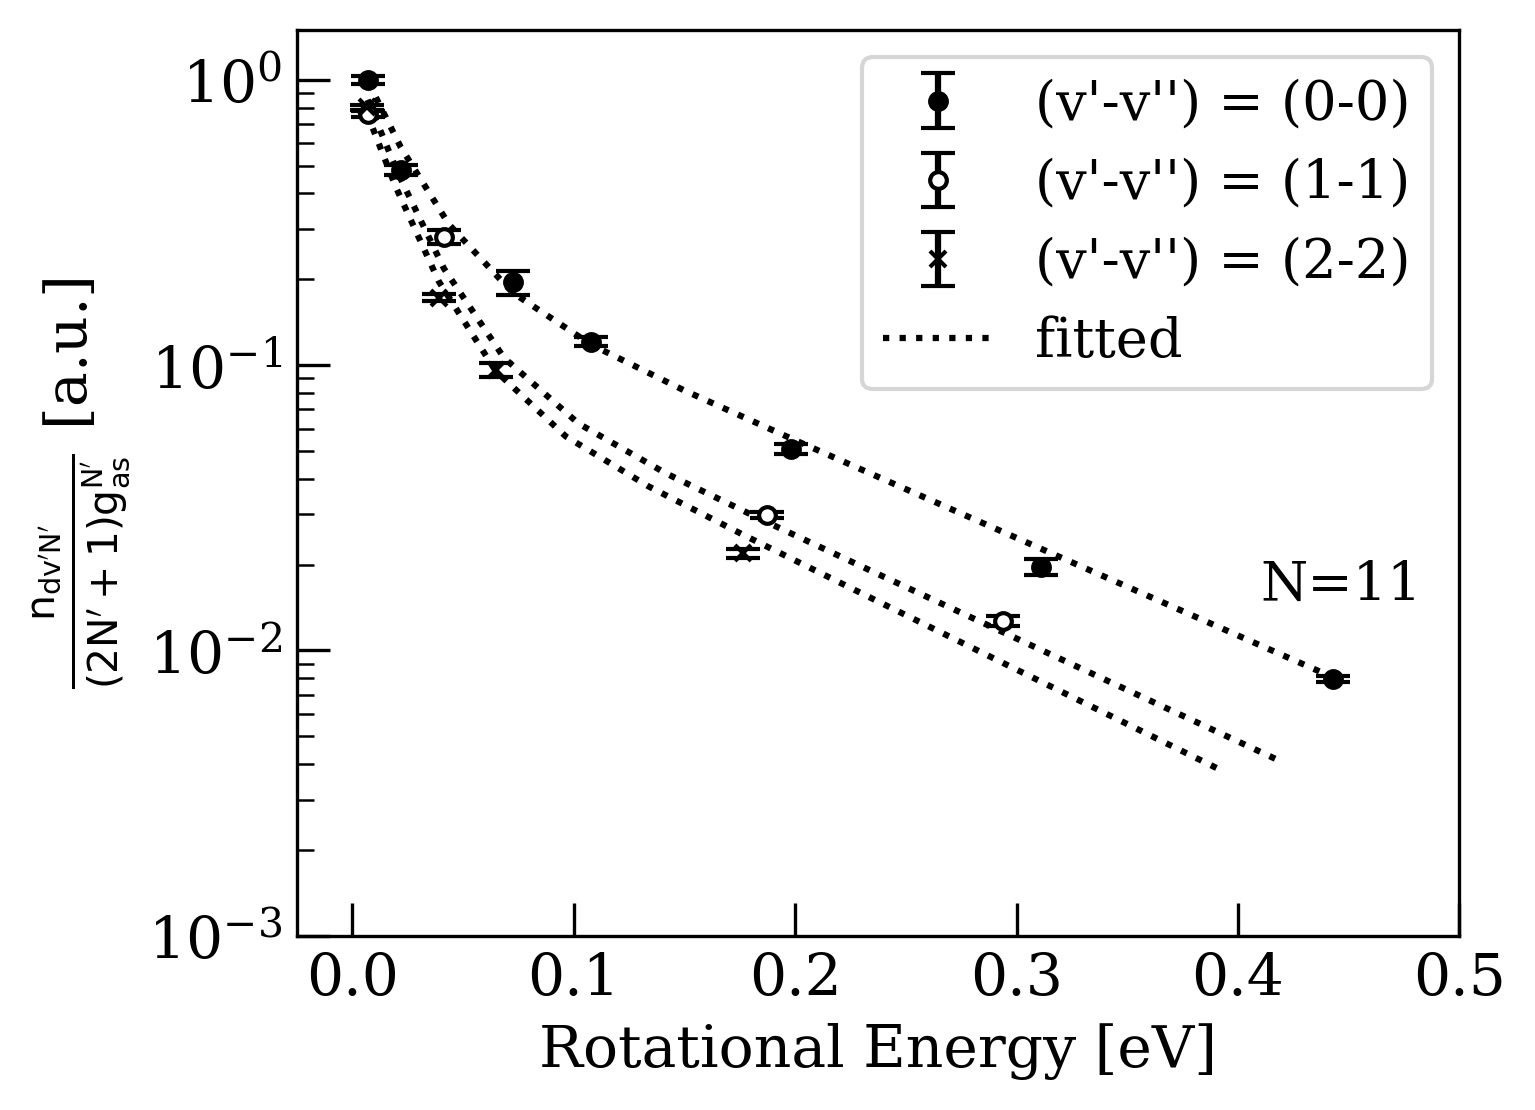
\includegraphics[width=15cm]{pictures/ishihara-upper-boltzmann.png}
    \caption[LHDでの発光上準位における振動・回転状態占有数の回転エネルギー依存性とその2温度ボルツマン分布の和によるフィッティング結果]{LHDでの発光上準位における振動・回転状態占有数の回転エネルギー依存性とその2温度ボルツマン分布の和によるフィッティング結果.図中の$N', N$はそれぞれ発光上準位及び基底準位の回転量子数であり,本論文の$J', J$に対応する.}
    \label{fig:ishihara-upper-boltzmann}
\end{figure}
